% What is built where, and the two firsts this project introduces.
%
% Both firsts are in the drawing and both are easy to get wrong. The
% module is the layer's first recipe that inherits the module class, and
% its package is not named after its recipe. The host tools are the first
% thing in this repository that is deliberately not in any image.
\documentclass[tikz, border=4pt]{standalone}
% Shared styles for the Project 9 figures.
%
% Every figure in this directory is standalone: it inputs this file and
% compiles on its own with
%
%     pdflatex arch.tex
%
% so a reader can render one drawing without building a book around it.
%
% The palette carries the distinction this project keeps confusing when it
% is drawn in one colour: what runs on the target, what runs on the host,
% and which of the two halves of the serial cable a given box is talking
% to. The fourth colour is for a fault that produces no symptom, which is
% three of the four faults here and the reason the project exists.
\usepackage{tikz}
\usepackage[siunitx]{circuitikz}
\usetikzlibrary{arrows.meta, backgrounds, calc, fit, positioning, shapes.geometric, shapes.misc}

\definecolor{usercol}{RGB}{222, 235, 247}   % target, user space
\definecolor{kerncol}{RGB}{198, 219, 239}   % target, kernel
\definecolor{hostcol}{RGB}{229, 245, 224}   % host, off the board
\definecolor{toolcol}{RGB}{254, 217, 118}   % a debugging tool
\definecolor{hwcol}{RGB}{229, 229, 229}     % hardware, files, RAM
\definecolor{quietcol}{RGB}{245, 245, 245}  % a fault with no symptom
\definecolor{linecol}{RGB}{70, 70, 70}
\definecolor{badcol}{RGB}{200, 60, 60}
\definecolor{okcol}{RGB}{60, 140, 70}

\tikzset{
  blk/.style   = {draw=linecol, rounded corners=2pt, align=center,
                  font=\sffamily\small, inner sep=4pt, minimum height=9mm},
  user/.style  = {blk, fill=usercol},
  kern/.style  = {blk, fill=kerncol},
  host/.style  = {blk, fill=hostcol},
  tool/.style  = {blk, fill=toolcol},
  hw/.style    = {blk, fill=hwcol},
  quiet/.style = {blk, fill=quietcol, draw=linecol!50, dashed},
  bad/.style   = {blk, fill=white, draw=badcol, thick, text=badcol},
  layer/.style = {draw=linecol!40, dashed, rounded corners=3pt, inner sep=6pt},
  layerlabel/.style = {font=\sffamily\scriptsize\bfseries, inner sep=2pt},
  lbl/.style   = {font=\sffamily\scriptsize, fill=white, inner sep=1pt},
  flow/.style  = {-{Stealth[length=2mm]}, draw=linecol, thick},
  bus/.style   = {{Stealth[length=2mm]}-{Stealth[length=2mm]}, draw=linecol,
                  thick},
  % The serial line is drawn thick and dark everywhere it appears, because
  % the single point of this project's host side is that it is one wire.
  wire/.style  = {{Stealth[length=2mm]}-{Stealth[length=2mm]}, draw=linecol,
                  very thick},
  % UML sequence
  actor/.style = {blk, fill=usercol, font=\sffamily\scriptsize,
                  minimum height=6mm},
  lifeline/.style = {draw=linecol!50, dashed},
  msg/.style   = {-{Stealth[length=1.6mm]}, draw=linecol},
  reply/.style = {-{Stealth[length=1.6mm]}, draw=linecol, dashed},
  umlnote/.style = {draw=linecol!60, fill=yellow!12, rounded corners=1pt,
                    font=\sffamily\scriptsize, align=left, inner sep=3pt},
  activation/.style = {draw=linecol, fill=usercol, minimum width=2mm},
  % decision tree
  qst/.style   = {draw=linecol, fill=white, diamond, aspect=2.6, align=center,
                  font=\sffamily\scriptsize, inner sep=1pt},
  ans/.style   = {font=\sffamily\scriptsize\itshape, inner sep=1pt},
  fix/.style   = {blk, fill=hostcol, font=\sffamily\scriptsize, align=left},
  trans/.style = {-{Stealth[length=1.6mm]}, draw=linecol},
  % fault matrix
  cell/.style  = {draw=linecol!40, minimum width=17mm, minimum height=7mm,
                  font=\sffamily\scriptsize, align=center},
  hit/.style   = {cell, fill=okcol!25},
  miss/.style  = {cell, fill=badcol!12, text=badcol},
  head/.style  = {cell, font=\sffamily\scriptsize\bfseries, fill=hwcol},
}


\begin{document}
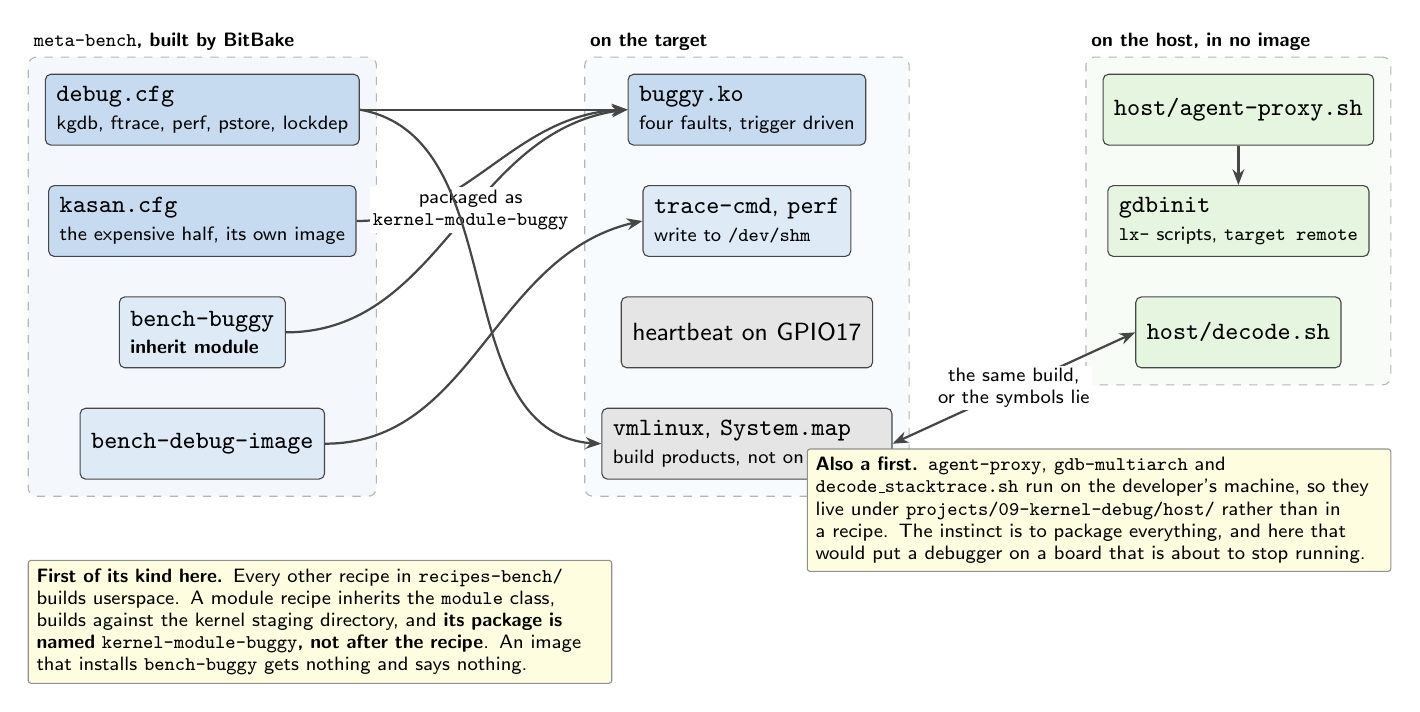
\begin{tikzpicture}[node distance=6mm, font=\sffamily\small]

  %% ---------------- the layer ----------------
  \node[kern, align=left] (dbg)
       {\texttt{debug.cfg}\\[-1pt]\scriptsize kgdb, ftrace, perf, pstore, lockdep};
  \node[kern, below=5mm of dbg, align=left] (kasan)
       {\texttt{kasan.cfg}\\[-1pt]\scriptsize the expensive half, its own image};
  \node[user, below=5mm of kasan, align=left] (rec)
       {\texttt{bench-buggy}\\[-1pt]\scriptsize \textbf{inherit module}};
  \node[user, below=5mm of rec, align=left] (img)
       {\texttt{bench-debug-image}};

  \begin{scope}[on background layer]
    \node[layer, fill=kerncol!20, fit=(dbg)(kasan)(rec)(img)] (lay) {};
  \end{scope}
  \node[layerlabel, anchor=south west] at (lay.north west)
       {\texttt{meta-bench}, built by BitBake};

  %% ---------------- on the target ----------------
  \node[kern, right=34mm of dbg, align=left] (ko)
       {\texttt{buggy.ko}\\[-1pt]\scriptsize four faults, trigger driven};
  \node[user, below=5mm of ko, align=left] (tools)
       {\texttt{trace-cmd}, \texttt{perf}\\[-1pt]\scriptsize write to \texttt{/dev/shm}};
  \node[hw, below=5mm of tools, align=left] (led)
       {heartbeat on GPIO17};
  \node[hw, below=5mm of led, align=left] (vm)
       {\texttt{vmlinux}, \texttt{System.map}\\[-1pt]
        \scriptsize build products, not on the card};

  \begin{scope}[on background layer]
    \node[layer, fill=usercol!20, fit=(ko)(tools)(led)(vm)] (tgt) {};
  \end{scope}
  \node[layerlabel, anchor=south west] at (tgt.north west) {on the target};

  %% ---------------- on the host ----------------
  \node[host, right=30mm of ko, align=left] (proxy)
       {\texttt{host/agent-proxy.sh}};
  \node[host, below=5mm of proxy, align=left] (gi)
       {\texttt{gdbinit}\\[-1pt]\scriptsize \texttt{lx-} scripts, \texttt{target remote}};
  \node[host, below=5mm of gi, align=left] (dec)
       {\texttt{host/decode.sh}};

  \begin{scope}[on background layer]
    \node[layer, fill=hostcol!30, fit=(proxy)(gi)(dec)] (hst) {};
  \end{scope}
  \node[layerlabel, anchor=south west] at (hst.north west)
       {on the host, \textbf{in no image}};

  %% ---------------- edges ----------------
  \draw[flow] (dbg.east) to[out=0, in=180] (ko.west);
  \draw[flow] (kasan.east) to[out=0, in=180] (ko.west);
  \draw[flow] (rec.east) to[out=0, in=185]
       node[lbl, pos=0.55, align=center]
       {packaged as\\\texttt{kernel-module-buggy}} (ko.west);
  \draw[flow] (img.east) to[out=0, in=190] (tools.west);
  \draw[flow] (dbg.east) to[out=-10, in=180] (vm.west);

  \draw[bus] (vm.east) -- node[lbl, align=center]
       {the same build,\\or the symbols lie} (dec.west);
  \draw[flow] (proxy) -- (gi);

  %% ---------------- the two notes ----------------
  \node[umlnote, anchor=north west, text width=72mm, align=left]
       at ($(lay.south west)+(0,-8mm)$)
       {\textbf{First of its kind here.} Every other recipe in
        \texttt{recipes-bench/} builds userspace. A module recipe inherits
        the \texttt{module} class, builds against the kernel staging
        directory, and \textbf{its package is named
        \texttt{kernel-module-buggy}, not after the recipe}. An image that
        installs \texttt{bench-buggy} gets nothing and says nothing.};

  \node[umlnote, anchor=north east, text width=72mm, align=left]
       at ($(hst.south east)+(0,-8mm)$)
       {\textbf{Also a first.} \texttt{agent-proxy}, \texttt{gdb-multiarch}
        and \texttt{decode\_stacktrace.sh} run on the developer's machine,
        so they live under \texttt{projects/09-kernel-debug/host/} rather
        than in a recipe. The instinct is to package everything, and here
        that would put a debugger on a board that is about to stop
        running.};

\end{tikzpicture}
\end{document}
